%%% The main file. It contains definitions of basic parameters and includes all other parts.

%% Settings for single-side (simplex) printing
% Margins: left 40mm, right 25mm, top and bottom 25mm
% (but beware, LaTeX adds 1in implicitly)
\documentclass[12pt,a4paper]{report}
\setlength\textwidth{145mm}
\setlength\textheight{247mm}
\setlength\oddsidemargin{15mm}
\setlength\evensidemargin{15mm}
\setlength\topmargin{0mm}
\setlength\headsep{0mm}
\setlength\headheight{0mm}
% \openright makes the following text appear on a right-hand page
\let\openright=\clearpage

%% Character encoding: usually latin2, cp1250 or utf8:
\usepackage[utf8]{inputenc}

%% Further useful packages (included in most LaTeX distributions)
\usepackage{amsmath}        % extensions for typesetting of math
\usepackage{amsfonts}       % math fonts
\usepackage{amsthm}         % theorems, definitions, etc.
%\usepackage{bbding}         % various symbols (squares, asterisks, scissors, ...)
\usepackage{bm}             % boldface symbols (\bm)
\usepackage{graphicx}       % embedding of pictures
\usepackage{fancyvrb}       % improved verbatim environment
%\usepackage{natbib}         % citation style AUTHOR (YEAR), or AUTHOR [NUMBER]
\usepackage[nottoc]{tocbibind} % makes sure that bibliography and the lists
			    % of figures/tables are included in the table
			    % of contents
\usepackage{dcolumn}        % improved alignment of table columns
\usepackage{booktabs}       % improved horizontal lines in tables
\usepackage{paralist}       % improved enumerate and itemize
\usepackage[usenames]{xcolor}  % typesetting in color
\usepackage{lineno}

% Definitions of macros (see description inside)
%%% This file contains definitions of various useful macros and environments %%%
%%% Please add more macros here instead of cluttering other files with them. %%%

%%% Minor tweaks of style

% These macros employ a little dirty trick to convince LaTeX to typeset
% chapter headings sanely, without lots of empty space above them.
% Feel free to ignore.
\makeatletter
\def\@makechapterhead#1{
  {\parindent \z@ \raggedright \normalfont
   \Huge\bfseries \thechapter. #1
   \par\nobreak
   \vskip 20\p@
}}
\def\@makeschapterhead#1{
  {\parindent \z@ \raggedright \normalfont
   \Huge\bfseries #1
   \par\nobreak
   \vskip 20\p@
}}
\makeatother

% This macro defines a chapter, which is not numbered, but is included
% in the table of contents.
\def\chapwithtoc#1{
\chapter*{#1}
\addcontentsline{toc}{chapter}{#1}
}

% Draw black "slugs" whenever a line overflows, so that we can spot it easily.
\overfullrule=1mm

%%% Macros for definitions, theorems, claims, examples, ... (requires amsthm package)

\theoremstyle{plain}
\newtheorem{thm}{Theorem}
\newtheorem{lemma}[thm]{Lemma}
\newtheorem{claim}[thm]{Claim}
\newtheorem{obs}[thm]{Observation}
\newtheorem{fct}[thm]{Fact}

\theoremstyle{definition}
\newtheorem{defn}{Definition}
\newtheorem{ntn}{Notation}

\theoremstyle{remark}
\newtheorem*{cor}{Corollary}
\newtheorem*{rem}{Remark}
\newtheorem*{example}{Example}

%%% An environment for proofs

%%% FIXME %%% \newenvironment{proof}{
%%% FIXME %%%   \par\medskip\noindent
%%% FIXME %%%   \textit{Proof}.
%%% FIXME %%% }{
%%% FIXME %%% \newline
%%% FIXME %%% \rightline{$\square$}  % or \SquareCastShadowBottomRight from bbding package
%%% FIXME %%% }

%%% An environment for typesetting of program code and input/output
%%% of programs. (Requires the fancyvrb package -- fancy verbatim.)

\DefineVerbatimEnvironment{code}{Verbatim}{fontsize=\small, frame=single}

%%% The field of all real and natural numbers
\newcommand{\R}{\mathbb{R}}
\newcommand{\N}{\mathbb{N}}

%%% Useful operators for statistics and probability
\DeclareMathOperator{\pr}{\textsf{P}}
\DeclareMathOperator{\E}{\textsf{E}\,}
\DeclareMathOperator{\var}{\textrm{var}}
\DeclareMathOperator{\sd}{\textrm{sd}}

%%% Transposition of a vector/matrix
\newcommand{\T}[1]{#1^\top}

%%% Various math goodies
\newcommand{\goto}{\rightarrow}
\newcommand{\gotop}{\stackrel{P}{\longrightarrow}}
\newcommand{\maon}[1]{o(n^{#1})}
\newcommand{\abs}[1]{\left|{#1}\right|}
\newcommand{\dint}{\int_0^\tau\!\!\int_0^\tau}
\newcommand{\isqr}[1]{\frac{1}{\sqrt{#1}}}

%%% Various table goodies
\newcommand{\pulrad}[1]{\raisebox{1.5ex}[0pt]{#1}}
\newcommand{\mc}[1]{\multicolumn{1}{c}{#1}}


\begin{document}
\linenumbers

\newsavebox{\smlmat}
\savebox{\smlmat}{$\left(\begin{smallmatrix}1&1\\1&0\end{smallmatrix}\right)$}
\newsavebox{\smlmatb}
\savebox{\smlmatb}{$\left(\begin{smallmatrix}1&1\\1&1\end{smallmatrix}\right)$}
\newsavebox{\smlmatc}
\savebox{\smlmatc}{$\left(\begin{smallmatrix}1&1&1\\0&1&0\end{smallmatrix}\right)$}

Throughout the paper, every time we speak about matrices we mean binary matrices and we omit the word binary. If we speak about a \emph{pattern}, we again mean a binary matrix and we use the word in order to distinguish among more matrices as well as to indicate relationship.

When dealing with matrices, we always index rows and column starting with zero and if we speak about a \emph{line}, we mean either a row or a column. When we order a set of line indices, we first put all rows, again starting with zero, and then all columns. For $M\in\{0,1\}^{m\times n}$, $[m]$ is a set of all row indices and $[m+n]$ is a set of all lines, where $m$-th element is an index of the first column.
\begin{ntn}
For $n\in\mathbb{N}$ let $[n]:=\{0,1,\dots,n-1\}$ and for $m\in\mathbb{N}$, where $n<m$ let $[n,m]:=\{n,n+1,\dots,m-1\}$.
\end{ntn}
\begin{ntn}
For an $m$ by $n$ matrix $M\in\{0,1\}^{m\times n}$ and $L\subseteq[m+n]$ let $M[L]$ denote a submatrix of $M$ induced by line indices in $L$.
\end{ntn}
\begin{ntn}
For an $m$ by $n$ matrix $M\in\{0,1\}^{m\times n}$, $R\subseteq[m]$ and $C\subseteq[n]$ let $M[R,C]$ denote a submatrix of $M$ induced by row indices in $R$ and column indices in $C$. Furthermore, for $r\in[m]$ and $c\in[n]$ let $M[r,c]:=M[\{r\},\{c\}]=M[\{r,c\}]$.
\end{ntn}
\begin{defn}
We say that a matrix $M\in\{0,1\}^{m\times n}$ \emph{contains} a pattern $P\in\{0,1\}^{h\times w}$ \emph{as a submatrix} and denote it by $P\leq M$ if there are $R\in[m]$ and $C\in[n]$ such that $|R|=h$ and $|C|=w$ for which for every $r\in R$ and $c\in C$ if $P[r,c]=1$, then $M[R,C][r,c]=1$.
\end{defn}
This does not necessarily mean $P=M[R,C]$ as $M[R,C]$ can have more one-entries than $P$ does.
\begin{ntn}
For an $m$ by $n$ matrix $M\in\{0,1\}^{m\times n}$ and $L\subseteq[m+n]$ in ascending order let $M_{\preceq}[L]$ denote a matrix acquired from $M$ by applying following operation for each $l\in L$:
\begin{itemize}
\item If $l$ is the first row index in $L$ replace the first $l+1$ rows by one row that is a bitwise or of replaced rows.
\item If $l$ is the first column index in $L$ replace the first $l+1$ columns by one column that is a bitwise or of replaced columns.
\item Otherwise, take $l$'s predecessor $l'\in L$ and replace lines $l'+1,l'+2,\dots,l$ by one line that is a bitwise or of replaced lines.
\end{itemize}
\end{ntn}
\begin{ntn}
For an $m$ by $n$ matrix $M\in\{0,1\}^{m\times n}$, $R\subseteq[m]$ and $C\subseteq[n]$ let $M_{\preceq}[R,C]:=M_{\preceq}[R\cup \{c+m|c\in C\}]$.
\end{ntn}
\textbf{Poznámka pro vedoucího:}

With this notation, for $M\in\{0,1\}^{m\times n}$ we have: $$M_{\preceq}[\{m,m+k\}]=M_{\preceq}[[m]\cup\{m,m+k,m+n-1\}]$$ This means that I always get a correct matrix and the definition of containing should be alright, but it is not very nice that it is ambiguous.
\begin{defn}
We say that a matrix $M\in\{0,1\}^{m\times n}$ \emph{contains} a pattern $P\in\{0,1\}^{h\times w}$ \emph{as an interval minor} and denote it by $P\preceq M$ if there are $R\in[m]$ and $C\in[n]$ such that $|R|=h$ and $|C|=w$ for which for every $r\in R$ and $c\in C$ if $P[r,c]=1$, then $M_{\preceq}[R,C][r,c]=1$.
\end{defn}
\begin{obs}
For all matrices $M$ and $P$, $P\leq M\Rightarrow P\preceq M$.
\end{obs}
\begin{obs}
For all matrices $M$ and $P$, if $P$ is a permutation matrix, then $P\leq M\Leftrightarrow P\preceq M$.
\end{obs}

\section{Characterizations}
\begin{defn}
For $M_1\in\{0,1\}^{n\times k}$, $M_2\in\{0,1\}^{n\times l}$ let $M\in\{0,1\}^{n\times k+l}$ be a \emph{horizontal join of} $M_1$ \emph{and} $M_2$, denoted by $M=M_1\oplus_hM_2$, if the first $k$ columns of $M$ give $M_1$ and the last $l$ columns of $M$ give $M_2$.
\end{defn}
\begin{defn}
A \emph{walk} in a matrix~$M$ is a sequence of some of its entries, beginning in the top left corner and ending in the bottom right one. If an entry at the position~$[i,j]$ is in the sequence, the next one is either $[i+1,j]$ or $[i,j+1]$.
\end{defn}
\begin{defn}
We call a binary matrix~$M$ a \emph{walking matrix} if there is a walk in $M$ such that all the one-entries of $M$ are contained on the walk.
\end{defn}

\subsection{Matrices of size $2\times2$}
\begin{thm}
Let $P=\left(\begin{smallmatrix}0&1\\1&0\end{smallmatrix}\right)$, then for all $M$: $P\not\preceq M\Leftrightarrow M$ is a walking matrix.
\end{thm}
\begin{proof}
Since $P$ is a permutation matrix, $P\not\preceq M\Leftrightarrow P\not\leq M$ and it is easy to see $P\not\leq M\Leftrightarrow M$ is a walking matrix.
\end{proof}
\begin{thm}
\label{theorem1}
Let $P=\left(\begin{smallmatrix}1&1\\1&0\end{smallmatrix}\right)$, then for all $M$: $P\not\preceq M\Leftrightarrow M$ looks like the matrix in Figure~\ref{p21}, where $M'$ is a walking matrix.
\end{thm}
\begin{figure}[h!]
\centering
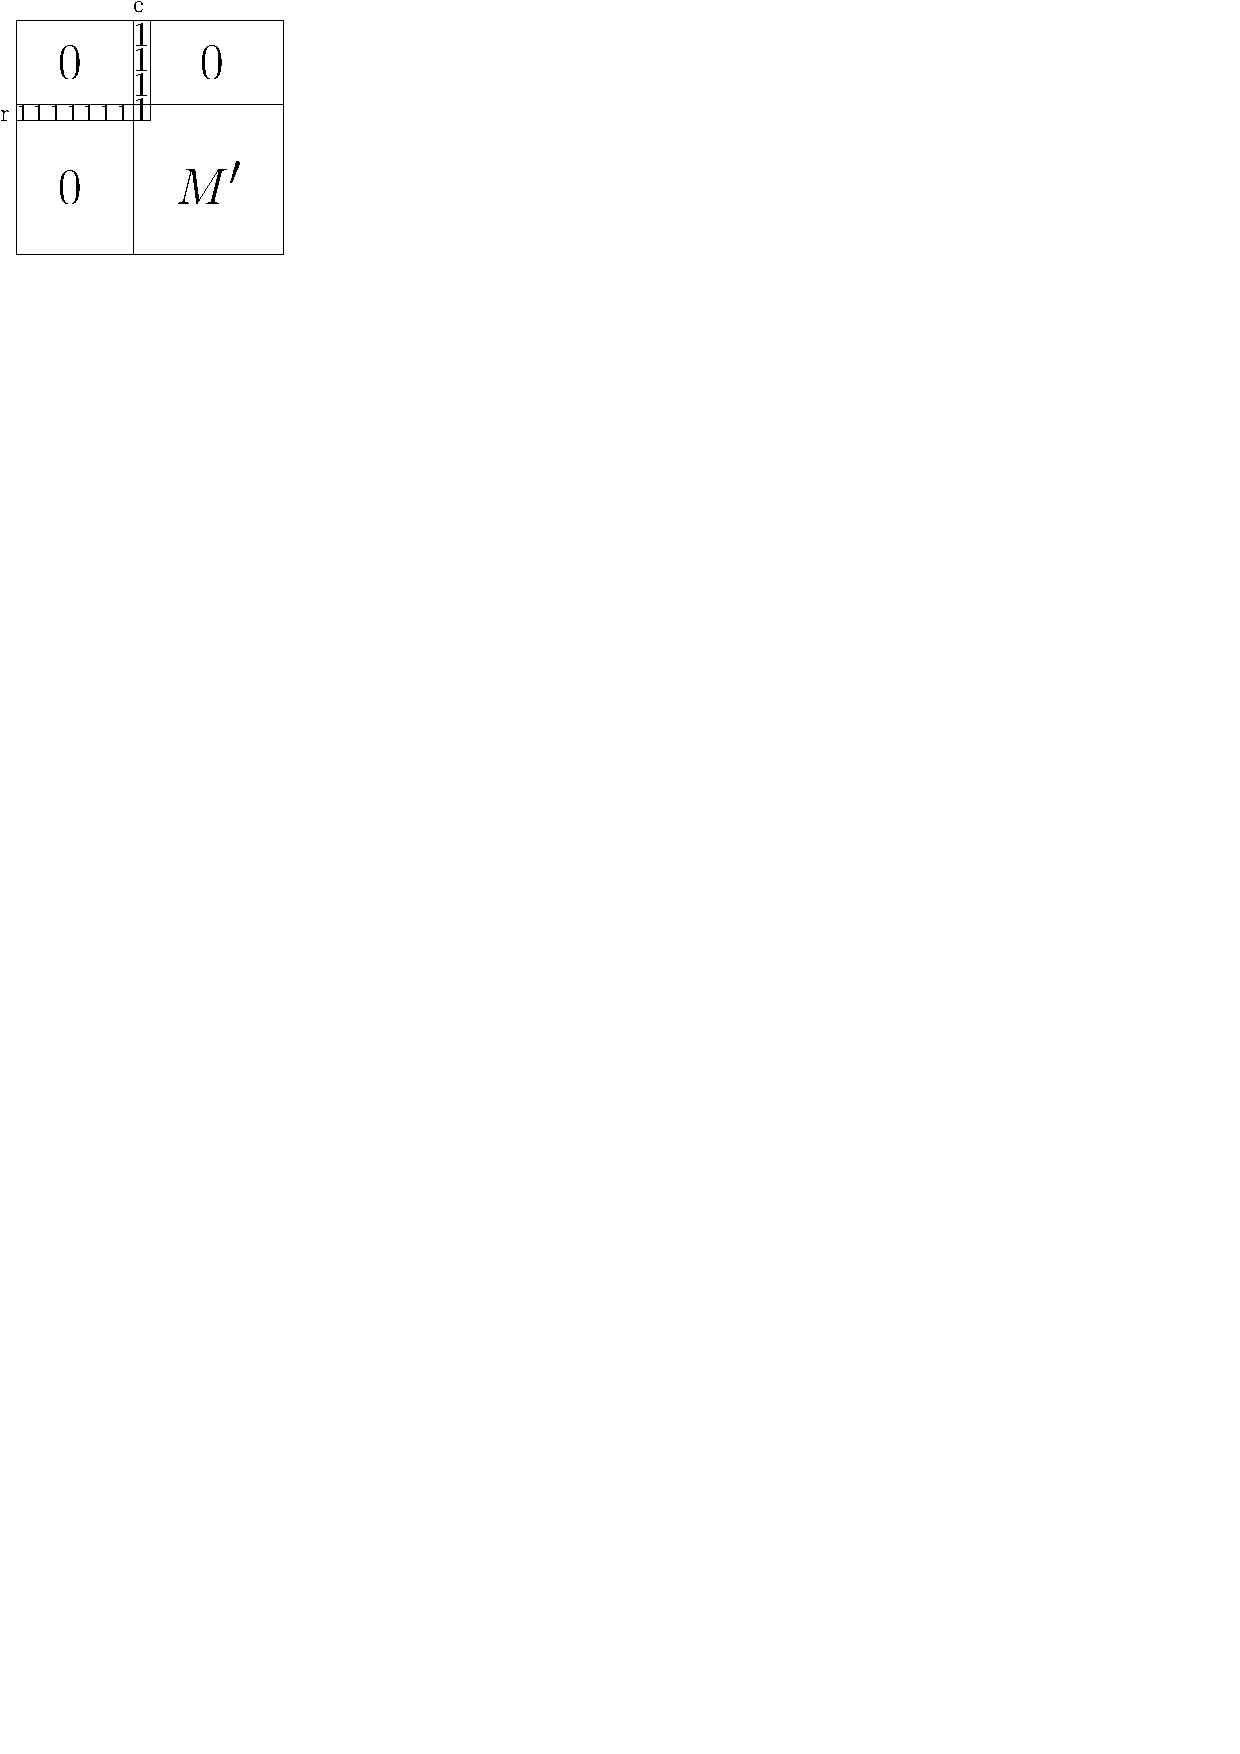
\includegraphics[width=60mm]{img/p21.pdf}
\caption{Characterization of a matrix avoiding \usebox{\smlmat} as an interval minor.}
\label{p21}
\end{figure}
\begin{proof}
\begin{itemize}
\item[$\Rightarrow$] If $\left(\begin{smallmatrix}0&1\\1&0\end{smallmatrix}\right)\not\preceq M$, then $M=M'$ and we are done. Else there are one-entries $M[r,c']$ and $M[r',c]$, where $r'<r$ and $c'<c$. If there was a one-entry in regions outside $M'$, the $r$-th row and the $c$-th column, then $P\preceq M$, which would be a contradiction. If $M'$ is not a walking matrix, then it contains $\left(\begin{smallmatrix}0&1\\1&0\end{smallmatrix}\right)$ and we again get a contradiction.
\item[$\Leftarrow$] For contradiction, assume that $M$ described in Figure~\ref{p21} contains $P$ as an interval minor. It means that there is a partition of the matrix into four quadrants such that there is at least one one-entry in each quadrant besides the bottom right one. If the matrix would be partitioned above the $r$-th row, then there would be only one column containing one-entries and it would not be possible for both top quadrants to have a one-entry. Similarly, if the matrix would be partitioned to the left of the $c$-th column, there would be only one row containing one-entries and there would not be one-entry in either top-left or bottom-left quadrant. Therefore, the partitioning lies bellow the $r$-th row and to the right of the $c$-th column, but if the quadrants contain one-entries, there is a $\left(\begin{smallmatrix}0&1\\1&0\end{smallmatrix}\right)$ interval minor in $M'$, which is a contradiction.
\end{itemize}
\end{proof}
\begin{lemma}
\label{lemma1}
TODO - lemma about existence of an element for which top-right and bottom-left submatrices are empty or symmetrically. I will need some kind of notation before I'm able to state and prove it. Was thinking about something like ``an element is ... if the submatrix $M[<r,>c]$ is empty''.
\end{lemma}
\begin{thm}
Let $P=\left(\begin{smallmatrix}1&1\\1&1\end{smallmatrix}\right)$, then for all $M$: $P\not\preceq M\Leftrightarrow M$ looks like one of the matrices in Figure~\ref{p22}, where $\left(\begin{smallmatrix}1&1\\1&0\end{smallmatrix}\right)\not\preceq M_1$, $\left(\begin{smallmatrix}0&1\\1&1\end{smallmatrix}\right)\not\preceq M_2$, $\left(\begin{smallmatrix}1&1\\0&1\end{smallmatrix}\right)\not\preceq M_3$ and  $\left(\begin{smallmatrix}1&0\\1&1\end{smallmatrix}\right)\not\preceq M_4$.
\end{thm}
\begin{figure}[h!]
\centering
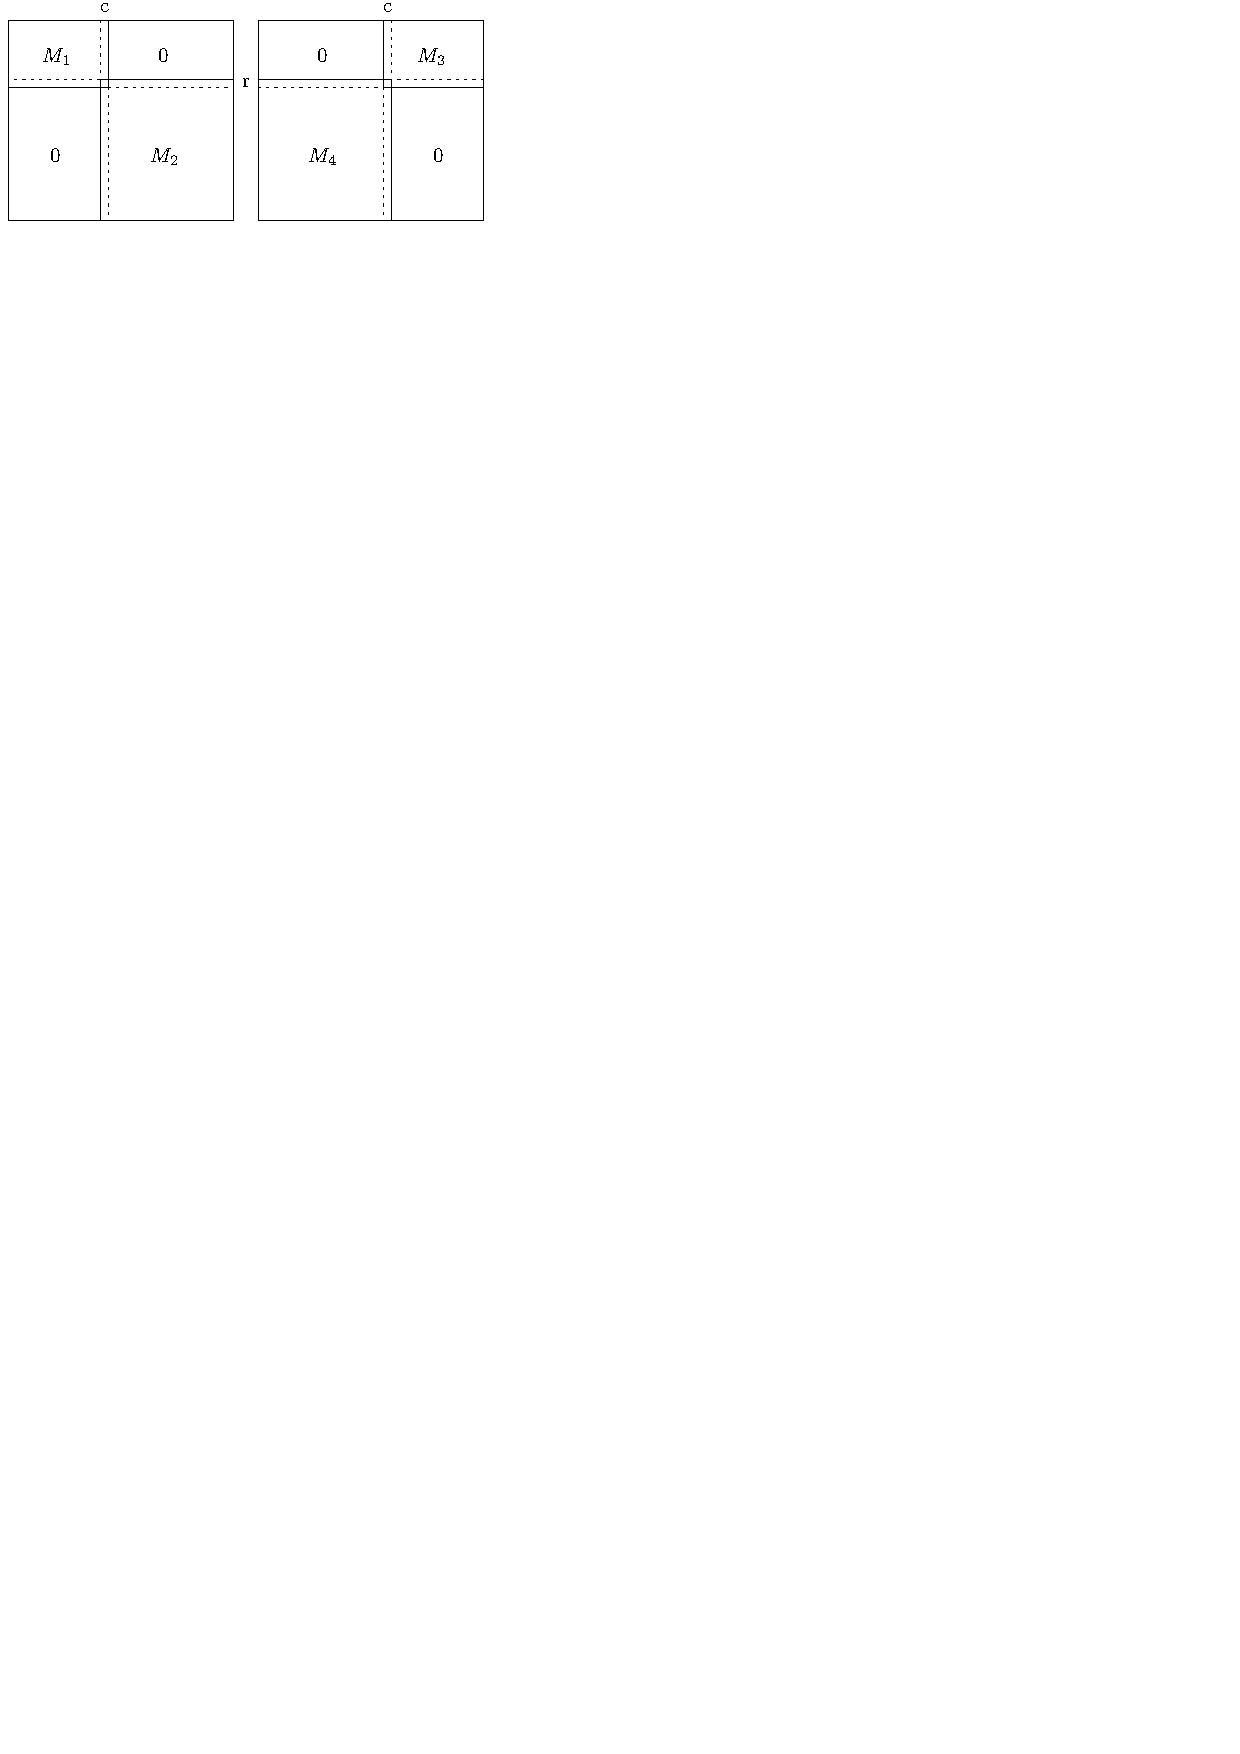
\includegraphics[height=60mm]{img/p22.pdf}
\caption{Characterization of a matrix avoiding \usebox{\smlmatb} as an interval minor.}
\label{p22}
\end{figure}
\begin{proof}
\item[$\Rightarrow$] We proceed by induction by the size of $M$.

If $M\in\{0,1\}^{2\times2}$, then it either avoids $\left(\begin{smallmatrix}0&1\\1&1\end{smallmatrix}\right)$ or $\left(\begin{smallmatrix}1&1\\1&0\end{smallmatrix}\right)$ and we are done.

For bigger $M$, there is, from Lemma~\ref{lemma1}, ``the element''. Assume the first case (top-right and bottom-left empty (will change this when I have some notation)). If $M_1$ is non-empty, then $\left(\begin{smallmatrix}0&1\\1&1\end{smallmatrix}\right)\not\preceq M_2$; otherwise, $P\preceq M$. Similarly, $\left(\begin{smallmatrix}1&1\\1&0\end{smallmatrix}\right)\not\preceq M_1$ if $M_2$ is non-empty. If one of them is empty, the other is a smaller matrix avoiding $P$ as an interval minor and by induction hypothesis, it can be partitioned. Adding empty rows and columns does not break any condition and we get a partitioning of the whole $M$.
\item[$\Leftarrow$] Let us assume $M$ looks like the left matrix in Figure~\ref{p22}, for the other one we would argue symmetrically. For contradiction, assume $P\preceq M$. In that case, we can partition $M$ into four quadrants such that there is at least one one-entry in each of them. It does not matter where we partition it, every time we either get $\left(\begin{smallmatrix}1&1\\1&0\end{smallmatrix}\right)\preceq M_1$ or $\left(\begin{smallmatrix}0&1\\1&1\end{smallmatrix}\right)\preceq M_2$, which is a contradiction.
\end{proof}

\subsection{Matrices of size $2\times3$}
\begin{thm}
Let $P=\left(\begin{smallmatrix}1&0&1\\0&1&0\end{smallmatrix}\right)$, then for all $M$: $P\not\preceq M\Leftrightarrow M=M_1\oplus_hM_2$, where $\left(\begin{smallmatrix}1&0\\0&1\end{smallmatrix}\right)\not\preceq M_1$ and $\left(\begin{smallmatrix}0&1\\1&0\end{smallmatrix}\right)\not\preceq M_2$.
\end{thm}
\begin{proof}
\begin{itemize}
\item[$\Rightarrow$] Let $e=[r,c]$ be the top-most one-entry of $M$. If there was $\left(\begin{smallmatrix}1&0\\0&1\end{smallmatrix}\right)$ as an interval minor in the first $c-1$ columns of $M$, together with $e$ it would be the whole $P$; therefore, it is not. If the rest of the columns besides the first $c-1$ avoid $\left(\begin{smallmatrix}0&1\\1&0\end{smallmatrix}\right)$ as an interval minor, we are done. Let us assume it is not the case and $e_{0,0},e_{1,1}$ be any two one-entries forming the forbidden pattern. Similarly, let the first $c$ columns contain $\left(\begin{smallmatrix}1&0\\0&1\end{smallmatrix}\right)$ as an interval minor (else $P\preceq M$) and $e_{0,1},e_{1,0}$ be any two one-entries forming the forbidden pattern. Now if we take $e_{0,0},e_{0,1}$ and a lower of $e_{1,0}$ and $e_{1,1}$ we get forbidden pattern $P$ as an interval minor, which is a contradiction. 
\item[$\Leftarrow$] For contradiction let us assume $P\preceq M$ and $M=M_1\oplus_hM_2$. If $P$ is an interval minor of $M$, let us look where is the one-entry of $M$, where the bottom one of $P$ can be mapped. If it is in $M_1$, then $P\not\preceq M$ because $\left(\begin{smallmatrix}0&1\\1&0\end{smallmatrix}\right)\not\preceq M_1$. Similarly, if it is in $M_2$, then $P\not\preceq M$ because $\left(\begin{smallmatrix}1&0\\0&1\end{smallmatrix}\right)\not\preceq M_2$.
\end{itemize}
\end{proof}
\begin{lemma}
\label{lemma2}
Let $P=\left(\begin{smallmatrix}1&1&1\\0&1&0\end{smallmatrix}\right)$, then for all $M$: $P\not\preceq M\Rightarrow M=M_1\oplus_hM_2$, where $\left(\begin{smallmatrix}1&1\\0&1\end{smallmatrix}\right)\not\preceq M_1$ and $\left(\begin{smallmatrix}0&1\\1&0\end{smallmatrix}\right)\not\preceq M_2$ or $\left(\begin{smallmatrix}1&0\\0&1\end{smallmatrix}\right)\not\preceq M_1$ and $\left(\begin{smallmatrix}1&1\\1&0\end{smallmatrix}\right)\not\preceq M_2$.
\end{lemma}
\begin{proof}
Let $e=[r,c]$ be the top-most one-entry of $M$. If there was $\left(\begin{smallmatrix}1&1\\0&1\end{smallmatrix}\right)$ as an interval minor in the first $c-1$ columns of $M$, together with $e$ it would be the whole $P$; therefore, it is not. Similarly, there is not $\left(\begin{smallmatrix}1&1\\1&0\end{smallmatrix}\right)$ as an interval minor in the rest of columns besides the first $c$. Now, in order not to decompose $M$, the first $c$ columns induce $\left(\begin{smallmatrix}1&0\\0&1\end{smallmatrix}\right)$ as an interval minor, where $e_{0,0}$ and $e_{1,1}$ (non of them equal to $e$, since $e$ lies in the top-right corner) are any two one-entries forming the pattern, and the rest of columns besides the first $c-1$ induce $\left(\begin{smallmatrix}0&1\\1&0\end{smallmatrix}\right)$ as an interval minor and $e_{0,1},e_{1,0}$ are any two one-entries forming the pattern. In that case $e_{0,0},e,e_{0,1}$ and a lower one of $e_{1,0}$ and $e_{1,1}$ give us the forbidden pattern $P$ as an interval minor, which is a contradiction; therefore there exists described decomposition of $M$.
\end{proof}
\begin{thm}
Let $P=\left(\begin{smallmatrix}1&1&1\\0&1&0\end{smallmatrix}\right)$, then for all $M$: $P\not\preceq M\Leftrightarrow M$ looks like the matrix in Figure~\ref{p52} and $\left(\begin{smallmatrix}1&0\\0&1\end{smallmatrix}\right)\not\preceq M_1$ and $\left(\begin{smallmatrix}0&1\\1&0\end{smallmatrix}\right)\not\preceq M_2$.
\end{thm}
\begin{figure}[h!]
\centering
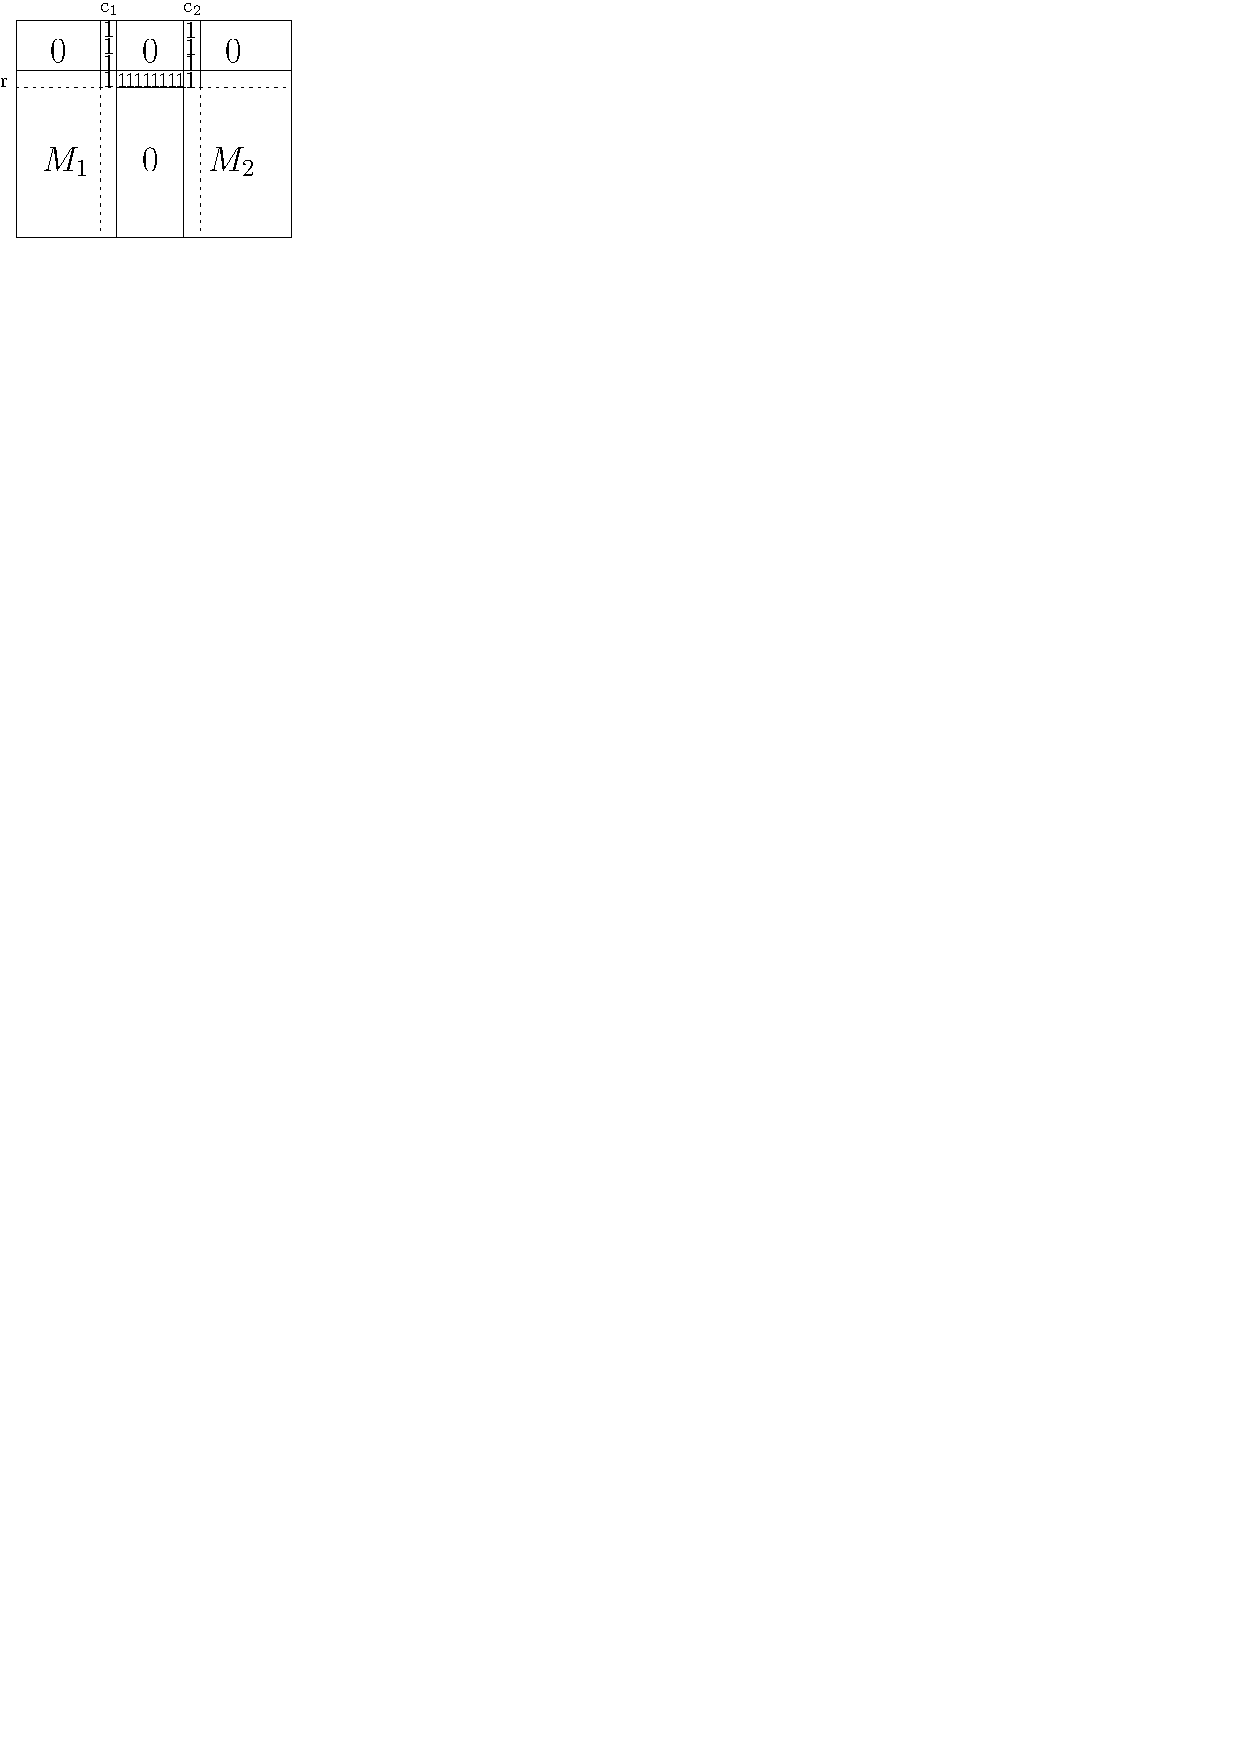
\includegraphics[height=60mm]{img/p52.pdf}
\caption{Characterization of a matrix avoiding \usebox{\smlmatb} as an interval minor.}
\label{p52}
\end{figure}
\begin{proof}
\begin{itemize}
\item[$\Rightarrow$] From Lemma~\ref{lemma2} we know $M=M_1'\oplus_hM_2'$, where $\left(\begin{smallmatrix}1&1\\0&1\end{smallmatrix}\right)\not\preceq M_1'$ and $\left(\begin{smallmatrix}0&1\\1&0\end{smallmatrix}\right)\not\preceq M_2'$. The other case would be dealt with similarly. As Theorem~\ref{theorem1} says, $M_1'$ can be characterized exactly like the first $c_2-1$ columns of $M$ and the rest then form a walking matrix. The only problem with our claim would be if there were two different columns having a one-entry above the $r$-th row. In that case those two one-entries together with a one-entry in the $r$-th row between the columns $c_1$ and $c_2$ and a one-entry in the $c_1$-th column above the $r$-th row form $P$ interval minor, which is a contradiction with $P\not\preceq M$.
\item[$\Leftarrow$] The bottom-middle one-entry of $P$ can not be mapped anywhere but to the $r$-th row, but in that case there are at most two columns having one-entries above it. (will do better hopefully)
\end{itemize}
\end{proof}

\section{Extremal function}
\begin{defn}
For a matrix $P$ and $n,m\in\mathbb{N}$ we define $Ex(P,m,n):=max\{\text{weight of }M|M\in\{0,1\}^{m\times n},P\not\leq M\}$. We denote $Ex(P,n):=Ex(P,n,n)$.
\end{defn}
\begin{defn}
For a matrix $P$ and $n,m\in\mathbb{N}$ we define $Ex_{\preceq}(P,m,n):=max\{\text{weight of }M|M\in\{0,1\}^{m\times n},P\not\preceq M\}$. We denote $Ex(P,n):=Ex(P,n,n)$.
\end{defn}
\begin{obs}
For all $P,m,n$; $Ex_{\preceq}(P,m,n)\leq Ex(P,m,n)$.
\end{obs}
\begin{obs}
If $P\in\{0,1\}^{k\times l}$ has a one-entry at position $[a,b]$, then $$Ex(P,m,n)\geq\Big\{\begin{array}{ll}
m\cdot n & k>m\vee l>m \\
(k-1)n+(l-1)m-(k-1)(l-1) & \text{otherwise.}
\end{array}$$
\end{obs}
\begin{obs}
The same holds for $Ex_{\preceq}(P,m,n).$
\end{obs}
\begin{defn}
$P\in\{0,1\}^{k\times l}$ is \emph{(strongly) minimalist} if
$$Ex(P,m,n)=\Big\{\begin{array}{ll}
m\cdot n & k>m\vee l>m \\
(k-1)n+(l-1)m-(k-1)(l-1) & \text{otherwise.}
\end{array}$$
\end{defn}
\begin{defn}
$P\in\{0,1\}^{k\times l}$ is \emph{weakly minimalist} if
$$Ex_{\preceq}(P,m,n)=\Big\{\begin{array}{ll}
m\cdot n & k>m\vee l>m \\
(k-1)n+(l-1)m-(k-1)(l-1) & \text{otherwise.}
\end{array}$$
\end{defn}
\begin{obs}
If $P$ is strongly minimalist, then $P$ is weakly minimalist.
\end{obs}
\begin{fct}
\begin{enumerate}
\item $\left(\begin{smallmatrix}1\end{smallmatrix}\right)$ is strongly minimalist.
\item If $P\in\{0,1\}^{k\times l}$ is strongly minimalist and there is a one-entry in the last row in the $c$-th column, then $P'\in\{0,1\}^{k+1\times l}$, which is created from $P$ by adding a new row having a one-entry only in the $c$-th row, is strongly minimalist.
\item If $P$ is strongly minimalist, then after changing a one-entry into a zero-entry it is still strongly minimalist.
\end{enumerate}
\end{fct}

\openright
\end{document}
